\documentclass[1p]{elsarticle_modified}
%\bibliographystyle{elsarticle-num}

%\usepackage[colorlinks]{hyperref}
%\usepackage{abbrmath_seonhwa} %\Abb, \Ascr, \Acal ,\Abf, \Afrak
\usepackage{amsfonts}
\usepackage{amssymb}
\usepackage{amsmath}
\usepackage{amsthm}
\usepackage{scalefnt}
\usepackage{amsbsy}
\usepackage{kotex}
\usepackage{caption}
\usepackage{subfig}
\usepackage{color}
\usepackage{graphicx}
\usepackage{xcolor} %% white, black, red, green, blue, cyan, magenta, yellow
\usepackage{float}
\usepackage{setspace}
\usepackage{hyperref}

\usepackage{tikz}
\usetikzlibrary{arrows}

\usepackage{multirow}
\usepackage{array} % fixed length table
\usepackage{hhline}

%%%%%%%%%%%%%%%%%%%%%
\makeatletter
\renewcommand*\env@matrix[1][\arraystretch]{%
	\edef\arraystretch{#1}%
	\hskip -\arraycolsep
	\let\@ifnextchar\new@ifnextchar
	\array{*\c@MaxMatrixCols c}}
\makeatother %https://tex.stackexchange.com/questions/14071/how-can-i-increase-the-line-spacing-in-a-matrix
%%%%%%%%%%%%%%%

\usepackage[normalem]{ulem}

\newcommand{\msout}[1]{\ifmmode\text{\sout{\ensuremath{#1}}}\else\sout{#1}\fi}
%SOURCE: \msout is \stkout macro in https://tex.stackexchange.com/questions/20609/strikeout-in-math-mode

\newcommand{\cancel}[1]{
	\ifmmode
	{\color{red}\msout{#1}}
	\else
	{\color{red}\sout{#1}}
	\fi
}

\newcommand{\add}[1]{
	{\color{blue}\uwave{#1}}
}

\newcommand{\replace}[2]{
	\ifmmode
	{\color{red}\msout{#1}}{\color{blue}\uwave{#2}}
	\else
	{\color{red}\sout{#1}}{\color{blue}\uwave{#2}}
	\fi
}

\newcommand{\Sol}{\mathcal{S}} %segment
\newcommand{\D}{D} %diagram
\newcommand{\A}{\mathcal{A}} %arc


%%%%%%%%%%%%%%%%%%%%%%%%%%%%%5 test

\def\sl{\operatorname{\textup{SL}}(2,\Cbb)}
\def\psl{\operatorname{\textup{PSL}}(2,\Cbb)}
\def\quan{\mkern 1mu \triangleright \mkern 1mu}

\theoremstyle{definition}
\newtheorem{thm}{Theorem}[section]
\newtheorem{prop}[thm]{Proposition}
\newtheorem{lem}[thm]{Lemma}
\newtheorem{ques}[thm]{Question}
\newtheorem{cor}[thm]{Corollary}
\newtheorem{defn}[thm]{Definition}
\newtheorem{exam}[thm]{Example}
\newtheorem{rmk}[thm]{Remark}
\newtheorem{alg}[thm]{Algorithm}

\newcommand{\I}{\sqrt{-1}}
\begin{document}

%\begin{frontmatter}
%
%\title{Boundary parabolic representations of knots up to 8 crossings}
%
%%% Group authors per affiliation:
%\author{Yunhi Cho} 
%\address{Department of Mathematics, University of Seoul, Seoul, Korea}
%\ead{yhcho@uos.ac.kr}
%
%
%\author{Seonhwa Kim} %\fnref{s_kim}}
%\address{Center for Geometry and Physics, Institute for Basic Science, Pohang, 37673, Korea}
%\ead{ryeona17@ibs.re.kr}
%
%\author{Hyuk Kim}
%\address{Department of Mathematical Sciences, Seoul National University, Seoul 08826, Korea}
%\ead{hyukkim@snu.ac.kr}
%
%\author{Seokbeom Yoon}
%\address{Department of Mathematical Sciences, Seoul National University, Seoul, 08826,  Korea}
%\ead{sbyoon15@snu.ac.kr}
%
%\begin{abstract}
%We find all boundary parabolic representation of knots up to 8 crossings.
%
%\end{abstract}
%\begin{keyword}
%    \MSC[2010] 57M25 
%\end{keyword}
%
%\end{frontmatter}

%\linenumbers
%\tableofcontents
%
\newcommand\colored[1]{\textcolor{white}{\rule[-0.35ex]{0.8em}{1.4ex}}\kern-0.8em\color{red} #1}%
%\newcommand\colored[1]{\textcolor{white}{ #1}\kern-2.17ex	\textcolor{white}{ #1}\kern-1.81ex	\textcolor{white}{ #1}\kern-2.15ex\color{red}#1	}

{\Large $\underline{10_{115}~(K10a_{94})}$}

\setlength{\tabcolsep}{10pt}
\renewcommand{\arraystretch}{1.6}
\vspace{1cm}\begin{tabular}{m{100pt}>{\centering\arraybackslash}m{274pt}}
\multirow{5}{120pt}{
	\centering
	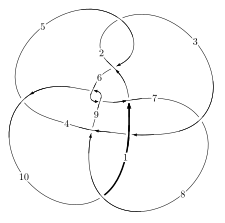
\includegraphics[width=112pt]{../../../GIT/diagram.site/Diagrams/png/199_10_115.png}\\
\ \ \ A knot diagram\footnotemark}&
\allowdisplaybreaks
\textbf{Linearized knot diagam} \\
\cline{2-2}
 &
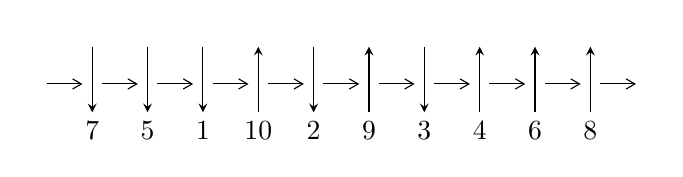
\begin{tikzpicture}[x=20pt, y=17pt]
	% nodes
	\node (C0) at (0, 0) {};
	\node (C1) at (1, 0) {};
	\node (C1U) at (1, +1) {};
	\node (C1D) at (1, -1) {7};

	\node (C2) at (2, 0) {};
	\node (C2U) at (2, +1) {};
	\node (C2D) at (2, -1) {5};

	\node (C3) at (3, 0) {};
	\node (C3U) at (3, +1) {};
	\node (C3D) at (3, -1) {1};

	\node (C4) at (4, 0) {};
	\node (C4U) at (4, +1) {};
	\node (C4D) at (4, -1) {10};

	\node (C5) at (5, 0) {};
	\node (C5U) at (5, +1) {};
	\node (C5D) at (5, -1) {2};

	\node (C6) at (6, 0) {};
	\node (C6U) at (6, +1) {};
	\node (C6D) at (6, -1) {9};

	\node (C7) at (7, 0) {};
	\node (C7U) at (7, +1) {};
	\node (C7D) at (7, -1) {3};

	\node (C8) at (8, 0) {};
	\node (C8U) at (8, +1) {};
	\node (C8D) at (8, -1) {4};

	\node (C9) at (9, 0) {};
	\node (C9U) at (9, +1) {};
	\node (C9D) at (9, -1) {6};

	\node (C10) at (10, 0) {};
	\node (C10U) at (10, +1) {};
	\node (C10D) at (10, -1) {8};
	\node (C11) at (11, 0) {};

	% arrows
	\draw[->,>={angle 60}]
	(C0) edge (C1) (C1) edge (C2) (C2) edge (C3) (C3) edge (C4) (C4) edge (C5) (C5) edge (C6) (C6) edge (C7) (C7) edge (C8) (C8) edge (C9) (C9) edge (C10) (C10) edge (C11) ;	\draw[->,>=stealth]
	(C1U) edge (C1D) (C2U) edge (C2D) (C3U) edge (C3D) (C4D) edge (C4U) (C5U) edge (C5D) (C6D) edge (C6U) (C7U) edge (C7D) (C8D) edge (C8U) (C9D) edge (C9U) (C10D) edge (C10U) ;
	\end{tikzpicture} \\
\hhline{~~} \\& 
\textbf{Solving Sequence} \\ \cline{2-2} 
 &
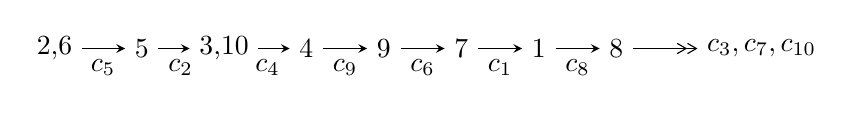
\begin{tikzpicture}[x=28pt, y=7pt]
	% node
	\node (A0) at (-1/8, 0) {2,6};
	\node (A1) at (1, 0) {5};
	\node (A2) at (33/16, 0) {3,10};
	\node (A3) at (25/8, 0) {4};
	\node (A4) at (33/8, 0) {9};
	\node (A5) at (41/8, 0) {7};
	\node (A6) at (49/8, 0) {1};
	\node (A7) at (57/8, 0) {8};
	\node (C1) at (1/2, -1) {$c_{5}$};
	\node (C2) at (3/2, -1) {$c_{2}$};
	\node (C3) at (21/8, -1) {$c_{4}$};
	\node (C4) at (29/8, -1) {$c_{9}$};
	\node (C5) at (37/8, -1) {$c_{6}$};
	\node (C6) at (45/8, -1) {$c_{1}$};
	\node (C7) at (53/8, -1) {$c_{8}$};
	\node (A8) at (9, 0) {$c_{3},c_{7},c_{10}$};

	% edge
	\draw[->,>=stealth]	
	(A0) edge (A1) (A1) edge (A2) (A2) edge (A3) (A3) edge (A4) (A4) edge (A5) (A5) edge (A6) (A6) edge (A7) ;
	\draw[->>,>={angle 60}]	
	(A7) edge (A8);
\end{tikzpicture} \\ 

\end{tabular} \\

\footnotetext{
The image of knot diagram is generated by the software ``\textbf{Draw programme}" developed by Andrew Bartholomew(\url{http://www.layer8.co.uk/maths/draw/index.htm\#Running-draw}), where we modified some parts for our purpose(\url{https://github.com/CATsTAILs/LinksPainter}).
}\phantom \\ \newline 
\centering \textbf{Ideals for irreducible components\footnotemark of $X_{\text{par}}$} 
 
\begin{align*}
I^u_{1}&=\langle 
1.34331\times10^{115} u^{65}+6.48169\times10^{115} u^{64}+\cdots+2.86473\times10^{116} b+1.11198\times10^{117},\\
\phantom{I^u_{1}}&\phantom{= \langle  }-1.40951\times10^{118} u^{65}-8.70781\times10^{118} u^{64}+\cdots+1.42377\times10^{119} a-1.81835\times10^{120},\\
\phantom{I^u_{1}}&\phantom{= \langle  }u^{66}+3 u^{65}+\cdots-77 u+21\rangle \\
I^u_{2}&=\langle 
- u^{11}-5 u^{10}-15 u^9-32 u^8-51 u^7-64 u^6-63 u^5-49 u^4-32 u^3-17 u^2+b-8 u-2,\\
\phantom{I^u_{2}}&\phantom{= \langle  }u^{11}+3 u^{10}+7 u^9+12 u^8+15 u^7+18 u^6+17 u^5+16 u^4+14 u^3+5 u^2+a+3 u-1,\\
\phantom{I^u_{2}}&\phantom{= \langle  }u^{12}+4 u^{11}+11 u^{10}+22 u^9+33 u^8+41 u^7+40 u^6+33 u^5+24 u^4+13 u^3+8 u^2+2 u+1\rangle \\
\\
\end{align*}
\raggedright * 2 irreducible components of $\dim_{\mathbb{C}}=0$, with total 78 representations.\\
\footnotetext{All coefficients of polynomials are rational numbers. But the coefficients are sometimes approximated in decimal forms when there is not enough margin.}
\newpage
\renewcommand{\arraystretch}{1}
\centering \section*{I. $I^u_{1}= \langle 1.34\times10^{115} u^{65}+6.48\times10^{115} u^{64}+\cdots+2.86\times10^{116} b+1.11\times10^{117},\;-1.41\times10^{118} u^{65}-8.71\times10^{118} u^{64}+\cdots+1.42\times10^{119} a-1.82\times10^{120},\;u^{66}+3 u^{65}+\cdots-77 u+21 \rangle$}
\flushleft \textbf{(i) Arc colorings}\\
\begin{tabular}{m{7pt} m{180pt} m{7pt} m{180pt} }
\flushright $a_{2}=$&$\begin{pmatrix}0\\u\end{pmatrix}$ \\
\flushright $a_{6}=$&$\begin{pmatrix}1\\0\end{pmatrix}$ \\
\flushright $a_{5}=$&$\begin{pmatrix}1\\- u^2\end{pmatrix}$ \\
\flushright $a_{3}=$&$\begin{pmatrix}- u\\u^3+u\end{pmatrix}$ \\
\flushright $a_{10}=$&$\begin{pmatrix}0.0989985 u^{65}+0.611601 u^{64}+\cdots-38.4442 u+12.7714\\-0.0468913 u^{65}-0.226258 u^{64}+\cdots+9.77991 u-3.88162\end{pmatrix}$ \\
\flushright $a_{4}=$&$\begin{pmatrix}-0.0379845 u^{65}+0.367680 u^{64}+\cdots-94.1129 u+27.5594\\0.0238215 u^{65}-0.0620212 u^{64}+\cdots+22.0119 u-6.47645\end{pmatrix}$ \\
\flushright $a_{9}=$&$\begin{pmatrix}0.145890 u^{65}+0.837859 u^{64}+\cdots-48.2241 u+16.6530\\-0.0468913 u^{65}-0.226258 u^{64}+\cdots+9.77991 u-3.88162\end{pmatrix}$ \\
\flushright $a_{7}=$&$\begin{pmatrix}0.183485 u^{65}+0.376814 u^{64}+\cdots+44.2181 u-10.0787\\-0.0938407 u^{65}-0.227660 u^{64}+\cdots-10.9063 u+3.96108\end{pmatrix}$ \\
\flushright $a_{1}=$&$\begin{pmatrix}0.431722 u^{65}+1.24657 u^{64}+\cdots+41.2616 u-2.40760\\0.0228165 u^{65}+0.142911 u^{64}+\cdots+2.85831 u-3.07897\end{pmatrix}$ \\
\flushright $a_{8}=$&$\begin{pmatrix}0.137406 u^{65}+0.154946 u^{64}+\cdots+52.6432 u-12.3398\\-0.106962 u^{65}-0.276610 u^{64}+\cdots-13.8597 u+4.46596\end{pmatrix}$\\&\end{tabular}
\flushleft \textbf{(ii) Obstruction class $= -1$}\\~\\
\flushleft \textbf{(iii) Cusp Shapes $= 0.703263 u^{65}+1.38008 u^{64}+\cdots+130.121 u-35.8005$}\\~\\
\newpage\renewcommand{\arraystretch}{1}
\flushleft \textbf{(iv) u-Polynomials at the component}\newline \\
\begin{tabular}{m{50pt}|m{274pt}}
Crossings & \hspace{64pt}u-Polynomials at each crossing \\
\hline $$\begin{aligned}c_{1}\end{aligned}$$&$\begin{aligned}
&u^{66}+u^{65}+\cdots-1128 u+193
\end{aligned}$\\
\hline $$\begin{aligned}c_{2},c_{5}\end{aligned}$$&$\begin{aligned}
&u^{66}+3 u^{65}+\cdots-77 u+21
\end{aligned}$\\
\hline $$\begin{aligned}c_{3}\end{aligned}$$&$\begin{aligned}
&u^{66}-5 u^{65}+\cdots-7 u+3
\end{aligned}$\\
\hline $$\begin{aligned}c_{4}\end{aligned}$$&$\begin{aligned}
&u^{66}- u^{65}+\cdots+1128 u+193
\end{aligned}$\\
\hline $$\begin{aligned}c_{6},c_{9}\end{aligned}$$&$\begin{aligned}
&u^{66}-3 u^{65}+\cdots+77 u+21
\end{aligned}$\\
\hline $$\begin{aligned}c_{7}\end{aligned}$$&$\begin{aligned}
&u^{66}- u^{65}+\cdots-31 u+3
\end{aligned}$\\
\hline $$\begin{aligned}c_{8}\end{aligned}$$&$\begin{aligned}
&u^{66}+u^{65}+\cdots+31 u+3
\end{aligned}$\\
\hline $$\begin{aligned}c_{10}\end{aligned}$$&$\begin{aligned}
&u^{66}+5 u^{65}+\cdots+7 u+3
\end{aligned}$\\
\hline
\end{tabular}\\~\\
\newpage\renewcommand{\arraystretch}{1}
\flushleft \textbf{(v) Riley Polynomials at the component}\newline \\
\begin{tabular}{m{50pt}|m{274pt}}
Crossings & \hspace{64pt}Riley Polynomials at each crossing \\
\hline $$\begin{aligned}c_{1},c_{4}\end{aligned}$$&$\begin{aligned}
&y^{66}+5 y^{65}+\cdots+1235072 y+37249
\end{aligned}$\\
\hline $$\begin{aligned}c_{2},c_{5},c_{6}\\c_{9}\end{aligned}$$&$\begin{aligned}
&y^{66}+35 y^{65}+\cdots+7259 y+441
\end{aligned}$\\
\hline $$\begin{aligned}c_{3},c_{10}\end{aligned}$$&$\begin{aligned}
&y^{66}+y^{65}+\cdots+149 y+9
\end{aligned}$\\
\hline $$\begin{aligned}c_{7},c_{8}\end{aligned}$$&$\begin{aligned}
&y^{66}+3 y^{65}+\cdots-31 y+9
\end{aligned}$\\
\hline
\end{tabular}\\~\\
\newpage\flushleft \textbf{(vi) Complex Volumes and Cusp Shapes}
$$\begin{array}{c|c|c}  
\text{Solutions to }I^u_{1}& \I (\text{vol} + \sqrt{-1}CS) & \text{Cusp shape}\\
 \hline 
\begin{aligned}
u &= -0.662737 + 0.747286 I \\
a &= \phantom{-}1.84867 - 0.18714 I \\
b &= \phantom{-}0.643705 + 0.913849 I\end{aligned}
 & -2.10904 + 4.58826 I & -5.96198 - 6.80019 I \\ \hline\begin{aligned}
u &= -0.662737 - 0.747286 I \\
a &= \phantom{-}1.84867 + 0.18714 I \\
b &= \phantom{-}0.643705 - 0.913849 I\end{aligned}
 & -2.10904 - 4.58826 I & -5.96198 + 6.80019 I \\ \hline\begin{aligned}
u &= -0.759989 + 0.676773 I \\
a &= \phantom{-}0.352294 - 0.243482 I \\
b &= \phantom{-}0.355245 - 1.033540 I\end{aligned}
 & -2.30167 + 0.78056 I & -4.09013 - 4.30344 I \\ \hline\begin{aligned}
u &= -0.759989 - 0.676773 I \\
a &= \phantom{-}0.352294 + 0.243482 I \\
b &= \phantom{-}0.355245 + 1.033540 I\end{aligned}
 & -2.30167 - 0.78056 I & -4.09013 + 4.30344 I \\ \hline\begin{aligned}
u &= \phantom{-}0.287386 + 0.983998 I \\
a &= -1.48006 - 0.92224 I \\
b &= -1.303580 - 0.315783 I\end{aligned}
 & \phantom{-}4.24208 - 0.93364 I & \phantom{-}15.9161 + 3.0658 I \\ \hline\begin{aligned}
u &= \phantom{-}0.287386 - 0.983998 I \\
a &= -1.48006 + 0.92224 I \\
b &= -1.303580 + 0.315783 I\end{aligned}
 & \phantom{-}4.24208 + 0.93364 I & \phantom{-}15.9161 - 3.0658 I \\ \hline\begin{aligned}
u &= \phantom{-}0.458890 + 0.841270 I \\
a &= \phantom{-}1.79291 - 0.60912 I \\
b &= \phantom{-}0.396945 - 1.221130 I\end{aligned}
 & -3.75920 + 1.29912 I & -3.74536 + 0.15014 I \\ \hline\begin{aligned}
u &= \phantom{-}0.458890 - 0.841270 I \\
a &= \phantom{-}1.79291 + 0.60912 I \\
b &= \phantom{-}0.396945 + 1.221130 I\end{aligned}
 & -3.75920 - 1.29912 I & -3.74536 - 0.15014 I \\ \hline\begin{aligned}
u &= -0.149058 + 1.034510 I \\
a &= -1.68613 + 0.22740 I \\
b &= -1.334980 + 0.373687 I\end{aligned}
 & \phantom{-}4.29717 + 0.35366 I & \phantom{-}9.83486 + 1.20455 I \\ \hline\begin{aligned}
u &= -0.149058 - 1.034510 I \\
a &= -1.68613 - 0.22740 I \\
b &= -1.334980 - 0.373687 I\end{aligned}
 & \phantom{-}4.29717 - 0.35366 I & \phantom{-}9.83486 - 1.20455 I\\
 \hline 
 \end{array}$$\newpage$$\begin{array}{c|c|c}  
\text{Solutions to }I^u_{1}& \I (\text{vol} + \sqrt{-1}CS) & \text{Cusp shape}\\
 \hline 
\begin{aligned}
u &= \phantom{-}0.355245 + 1.033540 I \\
a &= -0.362934 - 0.639915 I \\
b &= -0.759989 - 0.676773 I\end{aligned}
 & \phantom{-}2.30167 + 0.78056 I & \phantom{-0.000000 } 0 \\ \hline\begin{aligned}
u &= \phantom{-}0.355245 - 1.033540 I \\
a &= -0.362934 + 0.639915 I \\
b &= -0.759989 + 0.676773 I\end{aligned}
 & \phantom{-}2.30167 - 0.78056 I & \phantom{-0.000000 } 0 \\ \hline\begin{aligned}
u &= \phantom{-}0.643705 + 0.913849 I \\
a &= -1.20470 - 0.82212 I \\
b &= -0.662737 + 0.747286 I\end{aligned}
 & \phantom{-}2.10904 - 4.58826 I & \phantom{-0.000000 } 0 \\ \hline\begin{aligned}
u &= \phantom{-}0.643705 - 0.913849 I \\
a &= -1.20470 + 0.82212 I \\
b &= -0.662737 - 0.747286 I\end{aligned}
 & \phantom{-}2.10904 + 4.58826 I & \phantom{-0.000000 } 0 \\ \hline\begin{aligned}
u &= \phantom{-}0.360202 + 1.059140 I \\
a &= -2.20455 + 0.76831 I \\
b &= -0.342978 + 1.152930 I\end{aligned}
 & -2.39843 - 6.38163 I & \phantom{-0.000000 } 0 \\ \hline\begin{aligned}
u &= \phantom{-}0.360202 - 1.059140 I \\
a &= -2.20455 - 0.76831 I \\
b &= -0.342978 - 1.152930 I\end{aligned}
 & -2.39843 + 6.38163 I & \phantom{-0.000000 } 0 \\ \hline\begin{aligned}
u &= \phantom{-}0.359059 + 0.750855 I \\
a &= -0.298810 + 0.451021 I \\
b &= \phantom{-}0.08218 + 1.58909 I\end{aligned}
 & -4.14504 - 4.87522 I & -2.26179 + 9.07875 I \\ \hline\begin{aligned}
u &= \phantom{-}0.359059 - 0.750855 I \\
a &= -0.298810 - 0.451021 I \\
b &= \phantom{-}0.08218 - 1.58909 I\end{aligned}
 & -4.14504 + 4.87522 I & -2.26179 - 9.07875 I \\ \hline\begin{aligned}
u &= -0.783137 + 0.250577 I \\
a &= \phantom{-}0.259092 + 0.291154 I \\
b &= -0.271930 - 1.178510 I\end{aligned}
 & -3.01082 + 3.10826 I & -5.64725 - 5.61918 I \\ \hline\begin{aligned}
u &= -0.783137 - 0.250577 I \\
a &= \phantom{-}0.259092 - 0.291154 I \\
b &= -0.271930 + 1.178510 I\end{aligned}
 & -3.01082 - 3.10826 I & -5.64725 + 5.61918 I\\
 \hline 
 \end{array}$$\newpage$$\begin{array}{c|c|c}  
\text{Solutions to }I^u_{1}& \I (\text{vol} + \sqrt{-1}CS) & \text{Cusp shape}\\
 \hline 
\begin{aligned}
u &= -0.009834 + 0.802079 I \\
a &= -2.12400 - 0.10197 I \\
b &= -0.596579 + 1.045740 I\end{aligned}
 & \phantom{-}0.88395 - 2.01054 I & \phantom{-}3.45858 + 2.97810 I \\ \hline\begin{aligned}
u &= -0.009834 - 0.802079 I \\
a &= -2.12400 + 0.10197 I \\
b &= -0.596579 - 1.045740 I\end{aligned}
 & \phantom{-}0.88395 + 2.01054 I & \phantom{-}3.45858 - 2.97810 I \\ \hline\begin{aligned}
u &= -0.342978 + 1.152930 I \\
a &= \phantom{-}1.61910 - 0.70992 I \\
b &= \phantom{-}0.360202 + 1.059140 I\end{aligned}
 & \phantom{-}2.39843 + 6.38163 I & \phantom{-0.000000 } 0 \\ \hline\begin{aligned}
u &= -0.342978 - 1.152930 I \\
a &= \phantom{-}1.61910 + 0.70992 I \\
b &= \phantom{-}0.360202 - 1.059140 I\end{aligned}
 & \phantom{-}2.39843 - 6.38163 I & \phantom{-0.000000 } 0 \\ \hline\begin{aligned}
u &= -0.596579 + 1.045740 I \\
a &= \phantom{-}1.260790 + 0.175394 I \\
b &= -0.009834 + 0.802079 I\end{aligned}
 & -0.88395 + 2.01054 I & \phantom{-0.000000 } 0 \\ \hline\begin{aligned}
u &= -0.596579 - 1.045740 I \\
a &= \phantom{-}1.260790 - 0.175394 I \\
b &= -0.009834 - 0.802079 I\end{aligned}
 & -0.88395 - 2.01054 I & \phantom{-0.000000 } 0 \\ \hline\begin{aligned}
u &= -0.271930 + 1.178510 I \\
a &= -0.965808 - 0.442503 I \\
b &= -0.783137 - 0.250577 I\end{aligned}
 & \phantom{-}3.01082 + 3.10826 I & \phantom{-0.000000 } 0 \\ \hline\begin{aligned}
u &= -0.271930 - 1.178510 I \\
a &= -0.965808 + 0.442503 I \\
b &= -0.783137 + 0.250577 I\end{aligned}
 & \phantom{-}3.01082 - 3.10826 I & \phantom{-0.000000 } 0 \\ \hline\begin{aligned}
u &= \phantom{-}0.687231 + 0.358682 I \\
a &= \phantom{-}0.443779 + 0.395345 I \\
b &= -0.430277 - 1.187340 I\end{aligned}
 & -1.38542 + 3.12807 I & \phantom{-}0.18739 - 5.83461 I \\ \hline\begin{aligned}
u &= \phantom{-}0.687231 - 0.358682 I \\
a &= \phantom{-}0.443779 - 0.395345 I \\
b &= -0.430277 + 1.187340 I\end{aligned}
 & -1.38542 - 3.12807 I & \phantom{-}0.18739 + 5.83461 I\\
 \hline 
 \end{array}$$\newpage$$\begin{array}{c|c|c}  
\text{Solutions to }I^u_{1}& \I (\text{vol} + \sqrt{-1}CS) & \text{Cusp shape}\\
 \hline 
\begin{aligned}
u &= \phantom{-}0.542734 + 1.105870 I \\
a &= -1.71563 - 0.08154 I \\
b &= -0.68953 + 1.34019 I\end{aligned}
 & \phantom{-}0.80844 - 7.87674 I & \phantom{-0.000000 } 0 \\ \hline\begin{aligned}
u &= \phantom{-}0.542734 - 1.105870 I \\
a &= -1.71563 + 0.08154 I \\
b &= -0.68953 - 1.34019 I\end{aligned}
 & \phantom{-}0.80844 + 7.87674 I & \phantom{-0.000000 } 0 \\ \hline\begin{aligned}
u &= \phantom{-}1.195210 + 0.323364 I \\
a &= \phantom{-}0.164442 - 0.141775 I \\
b &= \phantom{-}0.499077 + 1.182910 I\end{aligned}
 & -3.08497 + 10.03660 I & \phantom{-0.000000 } 0 \\ \hline\begin{aligned}
u &= \phantom{-}1.195210 - 0.323364 I \\
a &= \phantom{-}0.164442 + 0.141775 I \\
b &= \phantom{-}0.499077 - 1.182910 I\end{aligned}
 & -3.08497 - 10.03660 I & \phantom{-0.000000 } 0 \\ \hline\begin{aligned}
u &= \phantom{-}0.734419 + 0.105022 I \\
a &= \phantom{-}0.549959 + 1.225450 I \\
b &= \phantom{-}0.734419 - 0.105022 I\end{aligned}
 & \phantom{-0.000000 -}5.41602 I & \phantom{-0.000000 } 0. - 4.57520 I \\ \hline\begin{aligned}
u &= \phantom{-}0.734419 - 0.105022 I \\
a &= \phantom{-}0.549959 - 1.225450 I \\
b &= \phantom{-}0.734419 + 0.105022 I\end{aligned}
 & \phantom{-0.000000 } -5.41602 I & \phantom{-0.000000 -}0. + 4.57520 I \\ \hline\begin{aligned}
u &= -0.430277 + 1.187340 I \\
a &= \phantom{-}1.052010 - 0.353445 I \\
b &= \phantom{-}0.687231 - 0.358682 I\end{aligned}
 & \phantom{-}1.38542 + 3.12807 I & \phantom{-0.000000 } 0 \\ \hline\begin{aligned}
u &= -0.430277 - 1.187340 I \\
a &= \phantom{-}1.052010 + 0.353445 I \\
b &= \phantom{-}0.687231 + 0.358682 I\end{aligned}
 & \phantom{-}1.38542 - 3.12807 I & \phantom{-0.000000 } 0 \\ \hline\begin{aligned}
u &= \phantom{-}0.499077 + 1.182910 I \\
a &= \phantom{-}1.205270 + 0.532515 I \\
b &= \phantom{-}1.195210 + 0.323364 I\end{aligned}
 & \phantom{-}3.08497 - 10.03660 I & \phantom{-0.000000 } 0 \\ \hline\begin{aligned}
u &= \phantom{-}0.499077 - 1.182910 I \\
a &= \phantom{-}1.205270 - 0.532515 I \\
b &= \phantom{-}1.195210 - 0.323364 I\end{aligned}
 & \phantom{-}3.08497 + 10.03660 I & \phantom{-0.000000 } 0\\
 \hline 
 \end{array}$$\newpage$$\begin{array}{c|c|c}  
\text{Solutions to }I^u_{1}& \I (\text{vol} + \sqrt{-1}CS) & \text{Cusp shape}\\
 \hline 
\begin{aligned}
u &= \phantom{-}0.396945 + 1.221130 I \\
a &= \phantom{-}1.047550 + 0.443482 I \\
b &= \phantom{-}0.458890 - 0.841270 I\end{aligned}
 & \phantom{-}3.75920 + 1.29912 I & \phantom{-0.000000 } 0 \\ \hline\begin{aligned}
u &= \phantom{-}0.396945 - 1.221130 I \\
a &= \phantom{-}1.047550 - 0.443482 I \\
b &= \phantom{-}0.458890 + 0.841270 I\end{aligned}
 & \phantom{-}3.75920 - 1.29912 I & \phantom{-0.000000 } 0 \\ \hline\begin{aligned}
u &= -0.610321 + 0.270672 I \\
a &= \phantom{-}0.749139 - 0.428729 I \\
b &= \phantom{-}0.290517 - 0.266226 I\end{aligned}
 & -1.36445 + 0.78938 I & -4.43693 - 1.27648 I \\ \hline\begin{aligned}
u &= -0.610321 - 0.270672 I \\
a &= \phantom{-}0.749139 + 0.428729 I \\
b &= \phantom{-}0.290517 + 0.266226 I\end{aligned}
 & -1.36445 - 0.78938 I & -4.43693 + 1.27648 I \\ \hline\begin{aligned}
u &= -0.448635 + 1.259820 I \\
a &= -1.39053 - 0.45102 I \\
b &= -0.71942 - 1.28265 I\end{aligned}
 & \phantom{-}1.26966 + 7.40298 I & \phantom{-0.000000 } 0 \\ \hline\begin{aligned}
u &= -0.448635 - 1.259820 I \\
a &= -1.39053 + 0.45102 I \\
b &= -0.71942 + 1.28265 I\end{aligned}
 & \phantom{-}1.26966 - 7.40298 I & \phantom{-0.000000 } 0 \\ \hline\begin{aligned}
u &= -1.303580 + 0.315783 I \\
a &= \phantom{-}0.334582 + 0.347965 I \\
b &= \phantom{-}0.287386 - 0.983998 I\end{aligned}
 & -4.24208 - 0.93364 I & \phantom{-0.000000 } 0 \\ \hline\begin{aligned}
u &= -1.303580 - 0.315783 I \\
a &= \phantom{-}0.334582 - 0.347965 I \\
b &= \phantom{-}0.287386 + 0.983998 I\end{aligned}
 & -4.24208 + 0.93364 I & \phantom{-0.000000 } 0 \\ \hline\begin{aligned}
u &= -0.043435 + 0.637728 I \\
a &= -4.04261 - 0.04501 I \\
b &= -0.043435 - 0.637728 I\end{aligned}
 & \phantom{-0.000000 } -4.25960 I & \phantom{-0.000000 }      -6
0. 10   - 0.329447 I \\ \hline\begin{aligned}
u &= -0.043435 - 0.637728 I \\
a &= -4.04261 + 0.04501 I \\
b &= -0.043435 + 0.637728 I\end{aligned}
 & \phantom{-0.000000 -}4.25960 I & \phantom{-0.000000 -}     -6
0. 10   + 0.329447 I\\
 \hline 
 \end{array}$$\newpage$$\begin{array}{c|c|c}  
\text{Solutions to }I^u_{1}& \I (\text{vol} + \sqrt{-1}CS) & \text{Cusp shape}\\
 \hline 
\begin{aligned}
u &= -1.334980 + 0.373687 I \\
a &= \phantom{-}0.207880 - 0.197593 I \\
b &= -0.149058 + 1.034510 I\end{aligned}
 & -4.29717 - 0.35366 I & \phantom{-0.000000 } 0 \\ \hline\begin{aligned}
u &= -1.334980 - 0.373687 I \\
a &= \phantom{-}0.207880 + 0.197593 I \\
b &= -0.149058 - 1.034510 I\end{aligned}
 & -4.29717 + 0.35366 I & \phantom{-0.000000 } 0 \\ \hline\begin{aligned}
u &= \phantom{-}0.280686 + 0.541514 I \\
a &= \phantom{-}0.076389 + 1.010860 I \\
b &= -0.198274 - 1.381690 I\end{aligned}
 & -4.11853 + 3.35398 I & -7.32610 + 2.92910 I \\ \hline\begin{aligned}
u &= \phantom{-}0.280686 - 0.541514 I \\
a &= \phantom{-}0.076389 - 1.010860 I \\
b &= -0.198274 + 1.381690 I\end{aligned}
 & -4.11853 - 3.35398 I & -7.32610 - 2.92910 I \\ \hline\begin{aligned}
u &= -0.198274 + 1.381690 I \\
a &= \phantom{-}0.457708 - 0.947576 I \\
b &= \phantom{-}0.280686 - 0.541514 I\end{aligned}
 & \phantom{-}4.11853 + 3.35398 I & \phantom{-0.000000 } 0 \\ \hline\begin{aligned}
u &= -0.198274 - 1.381690 I \\
a &= \phantom{-}0.457708 + 0.947576 I \\
b &= \phantom{-}0.280686 + 0.541514 I\end{aligned}
 & \phantom{-}4.11853 - 3.35398 I & \phantom{-0.000000 } 0 \\ \hline\begin{aligned}
u &= \phantom{-}0.68120 + 1.28817 I \\
a &= \phantom{-}1.52199 - 0.01935 I \\
b &= \phantom{-}0.68120 - 1.28817 I\end{aligned}
 & \phantom{-0.000000 } -16.6380 I & \phantom{-0.000000 } 0 \\ \hline\begin{aligned}
u &= \phantom{-}0.68120 - 1.28817 I \\
a &= \phantom{-}1.52199 + 0.01935 I \\
b &= \phantom{-}0.68120 + 1.28817 I\end{aligned}
 & \phantom{-0.000000 -}16.6380 I & \phantom{-0.000000 } 0 \\ \hline\begin{aligned}
u &= -0.71942 + 1.28265 I \\
a &= -0.971050 - 0.037443 I \\
b &= -0.448635 - 1.259820 I\end{aligned}
 & -1.26966 + 7.40298 I & \phantom{-0.000000 } 0 \\ \hline\begin{aligned}
u &= -0.71942 - 1.28265 I \\
a &= -0.971050 + 0.037443 I \\
b &= -0.448635 + 1.259820 I\end{aligned}
 & -1.26966 - 7.40298 I & \phantom{-0.000000 } 0\\
 \hline 
 \end{array}$$\newpage$$\begin{array}{c|c|c}  
\text{Solutions to }I^u_{1}& \I (\text{vol} + \sqrt{-1}CS) & \text{Cusp shape}\\
 \hline 
\begin{aligned}
u &= -0.68953 + 1.34019 I \\
a &= \phantom{-}1.43294 + 0.02037 I \\
b &= \phantom{-}0.542734 + 1.105870 I\end{aligned}
 & -0.80844 + 7.87674 I & \phantom{-0.000000 } 0 \\ \hline\begin{aligned}
u &= -0.68953 - 1.34019 I \\
a &= \phantom{-}1.43294 - 0.02037 I \\
b &= \phantom{-}0.542734 - 1.105870 I\end{aligned}
 & -0.80844 - 7.87674 I & \phantom{-0.000000 } 0 \\ \hline\begin{aligned}
u &= \phantom{-}0.08218 + 1.58909 I \\
a &= \phantom{-}0.412708 + 0.473001 I \\
b &= \phantom{-}0.359059 + 0.750855 I\end{aligned}
 & \phantom{-}4.14504 + 4.87522 I & \phantom{-0.000000 } 0 \\ \hline\begin{aligned}
u &= \phantom{-}0.08218 - 1.58909 I \\
a &= \phantom{-}0.412708 - 0.473001 I \\
b &= \phantom{-}0.359059 - 0.750855 I\end{aligned}
 & \phantom{-}4.14504 - 4.87522 I & \phantom{-0.000000 } 0 \\ \hline\begin{aligned}
u &= \phantom{-}0.290517 + 0.266226 I \\
a &= \phantom{-}0.824282 + 0.013319 I \\
b &= -0.610321 - 0.270672 I\end{aligned}
 & \phantom{-}1.36445 + 0.78938 I & \phantom{-}4.43693 - 1.27648 I \\ \hline\begin{aligned}
u &= \phantom{-}0.290517 - 0.266226 I \\
a &= \phantom{-}0.824282 - 0.013319 I \\
b &= -0.610321 + 0.270672 I\end{aligned}
 & \phantom{-}1.36445 - 0.78938 I & \phantom{-}4.43693 + 1.27648 I\\
 \hline 
 \end{array}$$\newpage\newpage\renewcommand{\arraystretch}{1}
\centering \section*{II. $I^u_{2}= \langle - u^{11}-5 u^{10}+\cdots+b-2,\;u^{11}+3 u^{10}+\cdots+a-1,\;u^{12}+4 u^{11}+\cdots+2 u+1 \rangle$}
\flushleft \textbf{(i) Arc colorings}\\
\begin{tabular}{m{7pt} m{180pt} m{7pt} m{180pt} }
\flushright $a_{2}=$&$\begin{pmatrix}0\\u\end{pmatrix}$ \\
\flushright $a_{6}=$&$\begin{pmatrix}1\\0\end{pmatrix}$ \\
\flushright $a_{5}=$&$\begin{pmatrix}1\\- u^2\end{pmatrix}$ \\
\flushright $a_{3}=$&$\begin{pmatrix}- u\\u^3+u\end{pmatrix}$ \\
\flushright $a_{10}=$&$\begin{pmatrix}- u^{11}-3 u^{10}+\cdots-3 u+1\\u^{11}+5 u^{10}+\cdots+8 u+2\end{pmatrix}$ \\
\flushright $a_{4}=$&$\begin{pmatrix}u^{11}+5 u^{10}+\cdots+14 u+5\\- u^{10}-4 u^9+\cdots-6 u-4\end{pmatrix}$ \\
\flushright $a_{9}=$&$\begin{pmatrix}-2 u^{11}-8 u^{10}+\cdots-11 u-1\\u^{11}+5 u^{10}+\cdots+8 u+2\end{pmatrix}$ \\
\flushright $a_{7}=$&$\begin{pmatrix}-2 u^{11}-10 u^{10}+\cdots-14 u-5\\-2 u^{11}-6 u^{10}+\cdots+2 u+4\end{pmatrix}$ \\
\flushright $a_{1}=$&$\begin{pmatrix}- u^{10}-4 u^9+\cdots-11 u-6\\- u^{11}-3 u^{10}+\cdots+2 u+4\end{pmatrix}$ \\
\flushright $a_{8}=$&$\begin{pmatrix}-3 u^{11}-13 u^{10}+\cdots-15 u-4\\- u^{11}-2 u^{10}+\cdots+4 u+4\end{pmatrix}$\\&\end{tabular}
\flushleft \textbf{(ii) Obstruction class $= 1$}\\~\\
\flushleft \textbf{(iii) Cusp Shapes $= 6 u^{11}+26 u^{10}+70 u^9+137 u^8+198 u^7+228 u^6+208 u^5+155 u^4+112 u^3+67 u^2+34 u+12$}\\~\\
\newpage\renewcommand{\arraystretch}{1}
\flushleft \textbf{(iv) u-Polynomials at the component}\newline \\
\begin{tabular}{m{50pt}|m{274pt}}
Crossings & \hspace{64pt}u-Polynomials at each crossing \\
\hline $$\begin{aligned}c_{1}\end{aligned}$$&$\begin{aligned}
&u^{12}-2 u^{10}+u^8-6 u^7+12 u^5+4 u^4-8 u^3+u^2+3 u+3
\end{aligned}$\\
\hline $$\begin{aligned}c_{2},c_{9}\end{aligned}$$&$\begin{aligned}
&u^{12}-4 u^{11}+\cdots-2 u+1
\end{aligned}$\\
\hline $$\begin{aligned}c_{3}\end{aligned}$$&$\begin{aligned}
&u^{12}+2 u^{11}- u^9+6 u^8+12 u^7+2 u^6-11 u^5-5 u^4+u^3+u^2+1
\end{aligned}$\\
\hline $$\begin{aligned}c_{4}\end{aligned}$$&$\begin{aligned}
&u^{12}-2 u^{10}+u^8+6 u^7-12 u^5+4 u^4+8 u^3+u^2-3 u+3
\end{aligned}$\\
\hline $$\begin{aligned}c_{5},c_{6}\end{aligned}$$&$\begin{aligned}
&u^{12}+4 u^{11}+\cdots+2 u+1
\end{aligned}$\\
\hline $$\begin{aligned}c_{7}\end{aligned}$$&$\begin{aligned}
&u^{12}+3 u^{10}+u^9+3 u^8+4 u^7+3 u^6+4 u^5+3 u^4+u^3+3 u^2+1
\end{aligned}$\\
\hline $$\begin{aligned}c_{8}\end{aligned}$$&$\begin{aligned}
&u^{12}+3 u^{10}- u^9+3 u^8-4 u^7+3 u^6-4 u^5+3 u^4- u^3+3 u^2+1
\end{aligned}$\\
\hline $$\begin{aligned}c_{10}\end{aligned}$$&$\begin{aligned}
&u^{12}-2 u^{11}+u^9+6 u^8-12 u^7+2 u^6+11 u^5-5 u^4- u^3+u^2+1
\end{aligned}$\\
\hline
\end{tabular}\\~\\
\newpage\renewcommand{\arraystretch}{1}
\flushleft \textbf{(v) Riley Polynomials at the component}\newline \\
\begin{tabular}{m{50pt}|m{274pt}}
Crossings & \hspace{64pt}Riley Polynomials at each crossing \\
\hline $$\begin{aligned}c_{1},c_{4}\end{aligned}$$&$\begin{aligned}
&y^{12}-4 y^{11}+\cdots-3 y+9
\end{aligned}$\\
\hline $$\begin{aligned}c_{2},c_{5},c_{6}\\c_{9}\end{aligned}$$&$\begin{aligned}
&y^{12}+6 y^{11}+\cdots+12 y+1
\end{aligned}$\\
\hline $$\begin{aligned}c_{3},c_{10}\end{aligned}$$&$\begin{aligned}
&y^{12}-4 y^{11}+\cdots+2 y+1
\end{aligned}$\\
\hline $$\begin{aligned}c_{7},c_{8}\end{aligned}$$&$\begin{aligned}
&y^{12}+6 y^{11}+\cdots+6 y+1
\end{aligned}$\\
\hline
\end{tabular}\\~\\
\newpage\flushleft \textbf{(vi) Complex Volumes and Cusp Shapes}
$$\begin{array}{c|c|c}  
\text{Solutions to }I^u_{2}& \I (\text{vol} + \sqrt{-1}CS) & \text{Cusp shape}\\
 \hline 
\begin{aligned}
u &= -0.238381 + 0.958097 I \\
a &= -1.64769 + 0.58255 I \\
b &= -1.340910 + 0.230586 I\end{aligned}
 & \phantom{-}3.76649 + 0.96528 I & -2.46025 - 6.19259 I \\ \hline\begin{aligned}
u &= -0.238381 - 0.958097 I \\
a &= -1.64769 - 0.58255 I \\
b &= -1.340910 - 0.230586 I\end{aligned}
 & \phantom{-}3.76649 - 0.96528 I & -2.46025 + 6.19259 I \\ \hline\begin{aligned}
u &= \phantom{-}0.275611 + 0.671814 I \\
a &= \phantom{-}3.49684 + 1.04213 I \\
b &= \phantom{-}0.275611 - 0.671814 I\end{aligned}
 & \phantom{-0.000000 } -4.91597 I & \phantom{-0.000000 -}0. + 11.11517 I \\ \hline\begin{aligned}
u &= \phantom{-}0.275611 - 0.671814 I \\
a &= \phantom{-}3.49684 - 1.04213 I \\
b &= \phantom{-}0.275611 + 0.671814 I\end{aligned}
 & \phantom{-0.000000 -}4.91597 I & \phantom{-0.000000 } 0. - 11.11517 I \\ \hline\begin{aligned}
u &= -0.540477 + 1.222060 I \\
a &= -1.42814 - 0.09893 I \\
b &= -0.540477 - 1.222060 I\end{aligned}
 & \phantom{-0.000000 -}6.92803 I & \phantom{-0.000000 } 0. - 5.92253 I \\ \hline\begin{aligned}
u &= -0.540477 - 1.222060 I \\
a &= -1.42814 + 0.09893 I \\
b &= -0.540477 + 1.222060 I\end{aligned}
 & \phantom{-0.000000 } -6.92803 I & \phantom{-0.000000 -}0. + 5.92253 I \\ \hline\begin{aligned}
u &= -1.340910 + 0.230586 I \\
a &= -0.144225 - 0.306569 I \\
b &= -0.238381 + 0.958097 I\end{aligned}
 & -3.76649 - 0.96528 I & \phantom{-}2.46025 + 6.19259 I \\ \hline\begin{aligned}
u &= -1.340910 - 0.230586 I \\
a &= -0.144225 + 0.306569 I \\
b &= -0.238381 - 0.958097 I\end{aligned}
 & -3.76649 + 0.96528 I & \phantom{-}2.46025 - 6.19259 I \\ \hline\begin{aligned}
u &= -0.09726 + 1.42673 I \\
a &= -0.530300 + 0.558704 I \\
b &= -0.058582 + 0.533279 I\end{aligned}
 & \phantom{-}3.74262 + 3.79217 I & -1.40025 - 6.58435 I \\ \hline\begin{aligned}
u &= -0.09726 - 1.42673 I \\
a &= -0.530300 - 0.558704 I \\
b &= -0.058582 - 0.533279 I\end{aligned}
 & \phantom{-}3.74262 - 3.79217 I & -1.40025 + 6.58435 I\\
 \hline 
 \end{array}$$\newpage$$\begin{array}{c|c|c}  
\text{Solutions to }I^u_{2}& \I (\text{vol} + \sqrt{-1}CS) & \text{Cusp shape}\\
 \hline 
\begin{aligned}
u &= -0.058582 + 0.533279 I \\
a &= \phantom{-}1.253520 - 0.119688 I \\
b &= -0.09726 + 1.42673 I\end{aligned}
 & -3.74262 - 3.79217 I & \phantom{-}1.40025 + 6.58435 I \\ \hline\begin{aligned}
u &= -0.058582 - 0.533279 I \\
a &= \phantom{-}1.253520 + 0.119688 I \\
b &= -0.09726 - 1.42673 I\end{aligned}
 & -3.74262 + 3.79217 I & \phantom{-}1.40025 - 6.58435 I\\
 \hline 
 \end{array}$$\newpage
\newpage\renewcommand{\arraystretch}{1}
\centering \section*{ III. u-Polynomials}
\begin{tabular}{m{50pt}|m{274pt}}
Crossings & \hspace{64pt}u-Polynomials at each crossing \\
\hline $$\begin{aligned}c_{1}\end{aligned}$$&$\begin{aligned}
&(u^{12}-2 u^{10}+u^8-6 u^7+12 u^5+4 u^4-8 u^3+u^2+3 u+3)\\
&\cdot(u^{66}+u^{65}+\cdots-1128 u+193)
\end{aligned}$\\
\hline $$\begin{aligned}c_{2}\end{aligned}$$&$\begin{aligned}
&(u^{12}-4 u^{11}+\cdots-2 u+1)(u^{66}+3 u^{65}+\cdots-77 u+21)
\end{aligned}$\\
\hline $$\begin{aligned}c_{3}\end{aligned}$$&$\begin{aligned}
&(u^{12}+2 u^{11}- u^9+6 u^8+12 u^7+2 u^6-11 u^5-5 u^4+u^3+u^2+1)\\
&\cdot(u^{66}-5 u^{65}+\cdots-7 u+3)
\end{aligned}$\\
\hline $$\begin{aligned}c_{4}\end{aligned}$$&$\begin{aligned}
&(u^{12}-2 u^{10}+u^8+6 u^7-12 u^5+4 u^4+8 u^3+u^2-3 u+3)\\
&\cdot(u^{66}- u^{65}+\cdots+1128 u+193)
\end{aligned}$\\
\hline $$\begin{aligned}c_{5}\end{aligned}$$&$\begin{aligned}
&(u^{12}+4 u^{11}+\cdots+2 u+1)(u^{66}+3 u^{65}+\cdots-77 u+21)
\end{aligned}$\\
\hline $$\begin{aligned}c_{6}\end{aligned}$$&$\begin{aligned}
&(u^{12}+4 u^{11}+\cdots+2 u+1)(u^{66}-3 u^{65}+\cdots+77 u+21)
\end{aligned}$\\
\hline $$\begin{aligned}c_{7}\end{aligned}$$&$\begin{aligned}
&(u^{12}+3 u^{10}+u^9+3 u^8+4 u^7+3 u^6+4 u^5+3 u^4+u^3+3 u^2+1)\\
&\cdot(u^{66}- u^{65}+\cdots-31 u+3)
\end{aligned}$\\
\hline $$\begin{aligned}c_{8}\end{aligned}$$&$\begin{aligned}
&(u^{12}+3 u^{10}- u^9+3 u^8-4 u^7+3 u^6-4 u^5+3 u^4- u^3+3 u^2+1)\\
&\cdot(u^{66}+u^{65}+\cdots+31 u+3)
\end{aligned}$\\
\hline $$\begin{aligned}c_{9}\end{aligned}$$&$\begin{aligned}
&(u^{12}-4 u^{11}+\cdots-2 u+1)(u^{66}-3 u^{65}+\cdots+77 u+21)
\end{aligned}$\\
\hline $$\begin{aligned}c_{10}\end{aligned}$$&$\begin{aligned}
&(u^{12}-2 u^{11}+u^9+6 u^8-12 u^7+2 u^6+11 u^5-5 u^4- u^3+u^2+1)\\
&\cdot(u^{66}+5 u^{65}+\cdots+7 u+3)
\end{aligned}$\\
\hline
\end{tabular}\newpage\renewcommand{\arraystretch}{1}
\centering \section*{ IV. Riley Polynomials}
\begin{tabular}{m{50pt}|m{274pt}}
Crossings & \hspace{64pt}Riley Polynomials at each crossing \\
\hline $$\begin{aligned}c_{1},c_{4}\end{aligned}$$&$\begin{aligned}
&(y^{12}-4 y^{11}+\cdots-3 y+9)(y^{66}+5 y^{65}+\cdots+1235072 y+37249)
\end{aligned}$\\
\hline $$\begin{aligned}c_{2},c_{5},c_{6}\\c_{9}\end{aligned}$$&$\begin{aligned}
&(y^{12}+6 y^{11}+\cdots+12 y+1)(y^{66}+35 y^{65}+\cdots+7259 y+441)
\end{aligned}$\\
\hline $$\begin{aligned}c_{3},c_{10}\end{aligned}$$&$\begin{aligned}
&(y^{12}-4 y^{11}+\cdots+2 y+1)(y^{66}+y^{65}+\cdots+149 y+9)
\end{aligned}$\\
\hline $$\begin{aligned}c_{7},c_{8}\end{aligned}$$&$\begin{aligned}
&(y^{12}+6 y^{11}+\cdots+6 y+1)(y^{66}+3 y^{65}+\cdots-31 y+9)
\end{aligned}$\\
\hline
\end{tabular}
\vskip 2pc
\end{document}